% =====================================================================
% Chapter 5: BLEND
%
% Required topic: the description of the methodology, formally.
%
% The text is the section of the paper named after the tool, word for
% word, whose paragraphs are Overview, Perturbation-Difference
% Interval, Zonotope Bound Tightening, Conditional-Triangle
% Relaxation, Warm Start and Additional Techniques. Only the structure
% is adapted: the section becomes a chapter and its paragraphs become
% sections, the displayed formulas the lemmas refer to are numbered,
% and the perturbed input is written x^p throughout, as in the rest of
% the thesis, where the paper writes x'.
%
% Two parts come from elsewhere in the paper: the algorithm and its
% walkthrough, from sections/sec_appendix_algorithm.tex, and the two
% lemmas of the relaxation with their proofs, from
% sections/sec_appendix_soundness.tex, both word for word as well.
%
% fig_pipeline.pdf is copied from the figures of the paper.
% =====================================================================
\chapter{\tool: A Global Robustness Verifier}
\label{ch:blend}

In this chapter, we present our verifier, \tool. We begin with its overview and then define its main
components.

\section{Overview}
\label{sec:blend-overview}

\begin{figure}[t]
 \centering
 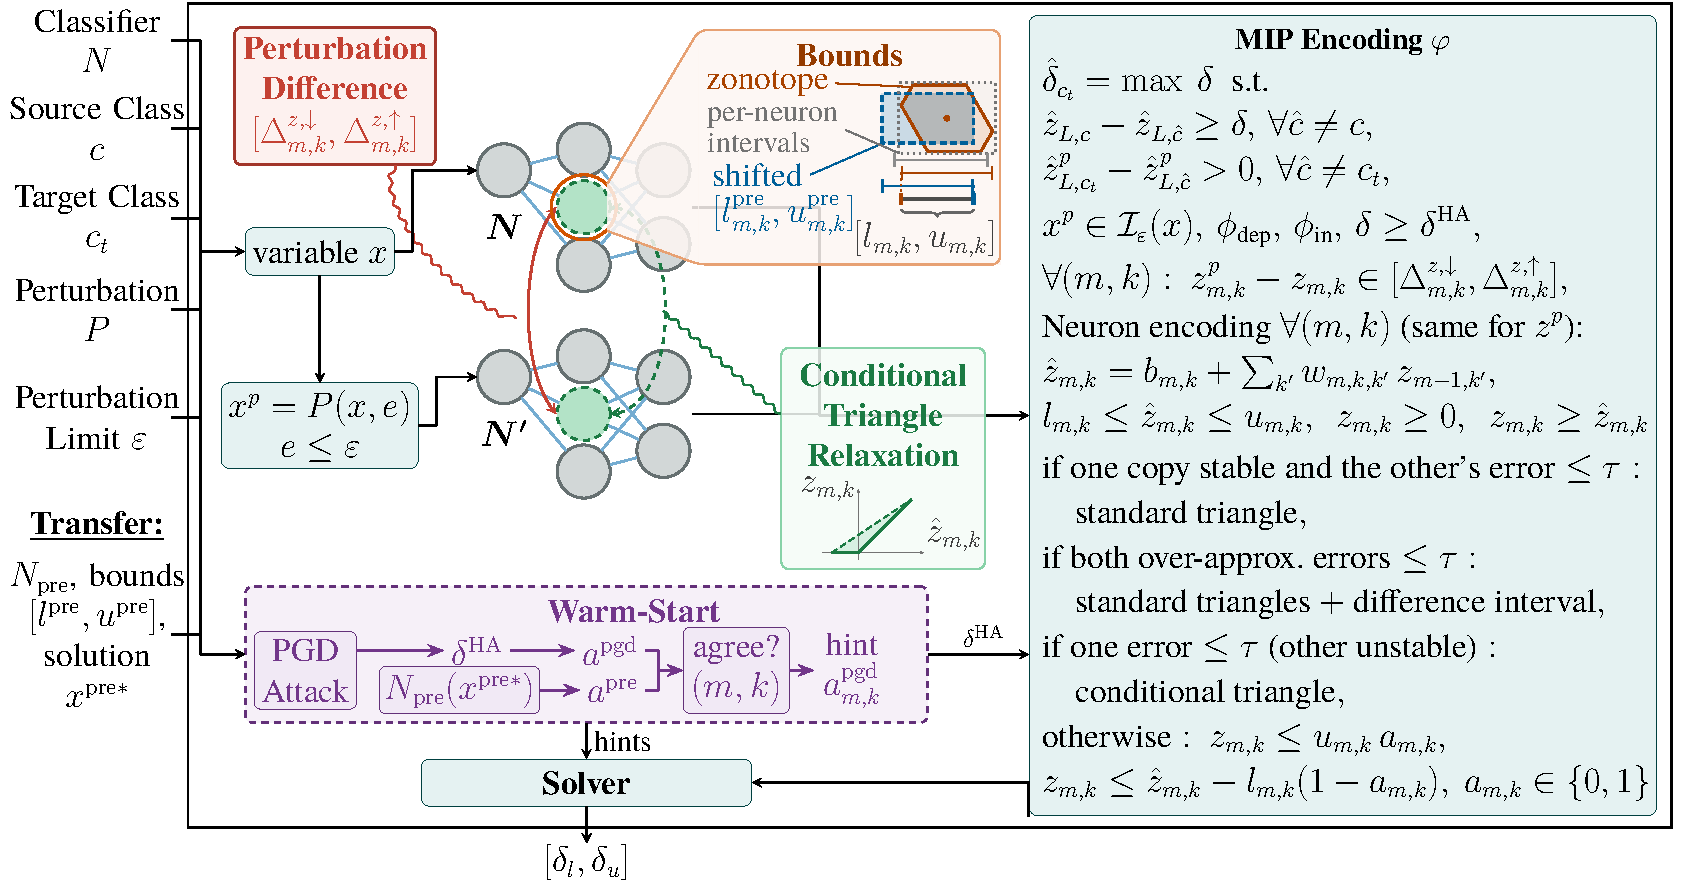
\includegraphics[width=\linewidth]{fig_pipeline}
 \caption{\tool leverages perturbation-difference intervals, zonotope bounds, a novel relaxation, and incremental verification.}
 \label{fig:pipeline}
\end{figure}

Figure~\ref{fig:pipeline} shows \tool's system. \tool takes a classifier $N$, a
source class $c$ and a target class $c_t$, and a perturbation $P$ of limit $\ep$. It returns the maximal
non-robust bound $\hat\delta_{c_t}$, or an interval $[\delta_l,\delta_u]$ bounding it if it reaches a
user-specified timeout. It supports a \emph{transfer mode} for incremental verification, where its
inputs also include a previously verified network $\Npre$ of the same architecture but possibly
different weights, together with $\Npre$'s analysis result: its verified per-neuron bounds
$[l^{\mathrm{pre}}_{m,k},u^{\mathrm{pre}}_{m,k}]$ and $[l^{p,\mathrm{pre}}_{m,k},u^{p,\mathrm{pre}}_{m,k}]$,
and the optimal input $x^{\mathrm{pre}*}$ of its solution. To compute the bound, \tool constructs a mixed-integer program (MIP) $\varphi$ whose
optimum is $\hat\delta_{c_t}$, building it layer by layer and finally submitting it to an off-the-shelf
solver. It begins by introducing a variable $x\in[0,1]^n$ for $N$'s input and
constraining the perturbed copy's input by $x^{p}=P(x,e)$ with $e\le\ep$ and $x^{p}\in[0,1]^n$. Then, for
every subsequent layer, it begins by computing, for each neuron, two bounds: a perturbation-difference
interval, bounding how far the perturbation shifts the neuron from its clean value, and a zonotope value
bound, tightening the neuron's range. In transfer mode, it further tightens each copy's bound by
intersecting it with $\Npre$'s verified bounds shifted by a difference zonotope. It then encodes each
neuron according to its bound
$[l_{m,k},u_{m,k}]$, and similarly $[l^{p}_{m,k},u^{p}_{m,k}]$: if the bound decides the ReLU, that is
$z_{m,k}=\hat z_{m,k}$ or $z_{m,k}=0$, it adds a linear constraint; if the bound is near-decided, it adds
a triangle or conditional-triangle relaxation; otherwise it adds a binary variable and the constraints defined by
\citet{tjeng2019}. Additionally, it adds the perturbation-difference interval and the zonotope bounds
to $\varphi$ to prune its search space. In parallel, \tool runs a PGD hyper-attack, as in \baseline~\cite{kabaha2024vhagar}, that yields a
feasible solution, whose objective lower-bounds $\hat\delta_{c_t}$, which is added to $\varphi$ to prune
the search space. The attack also yields per-neuron phase hints that warm-start the solver, guiding the initial setting of
its binaries. In transfer mode, \tool looks at the activation phase of every neuron at $\Npre$'s optimal solution $x^{\mathrm{pre}*}$ and decides its hint by checking agreement with the hyper-attack.

\begin{algorithm}[t]
\small
\caption{\protect\BLEND{$N$, $c$, $c_t$, $P$, $\ep$, $\Npre$}}\label{alg:blend}
\KwIn{classifier $N$; source class $c$, target class $c_t$; perturbation $P$ and limit $\ep$; and, in transfer mode, $\Npre$ with its verified bounds $[l^{\mathrm{pre}}_{m,k},u^{\mathrm{pre}}_{m,k}]$ and $[l^{p,\mathrm{pre}}_{m,k},u^{p,\mathrm{pre}}_{m,k}]$, and optimal input $x^{\mathrm{pre}*}$}
\KwOut{anytime bounds $[\delta_l,\delta_u]$ for the problem's objective, where $\delta_u$ soundly upper-bounds $\hat\delta_{c_t}$ when $\tau>0$}
$\varphi=$ MIP encoding of $N(x),N(x^{p})$\;
$(\delta^{\mathrm{HA}},a^{\mathrm{pgd}})=\PGD{$N,c,c_t,P,\ep$}$\;
$\varphi\wedge\{\hat\delta_{c_t}\ge\delta^{\mathrm{HA}}\}$\;
$\Delta^{z}_{0}=$ the gap between $x^{p}$ and $x$ under $P$\;
\For{$m=1$ \KwTo $L$}{
 \For{$k=1$ \KwTo $k_m$}{
  $\Delta^{\hat z}_{m,k}=\textstyle\sum_{k'} w_{m,k,k'}\,\Delta^{z}_{m-1,k'}$\;
  $[l_{m,k},u_{m,k}]$${}=[l^{p}_{m,k},u^{p}_{m,k}]$${}=$ zonotope bounds of $\hat z_{m,k}$ and $\hat z^{p}_{m,k}$\;
  $[d^\downarrow_{m,k},d^\uparrow_{m,k}]=$ difference-zonotope bounds\;
  $[l_{m,k},u_{m,k}]=[l_{m,k},u_{m,k}]\cap([l^{\mathrm{pre}}_{m,k},u^{\mathrm{pre}}_{m,k}]+[d^\downarrow_{m,k},d^\uparrow_{m,k}])$\;
  $[l^{p}_{m,k},u^{p}_{m,k}]=[l^{p}_{m,k},u^{p}_{m,k}]\cap([l^{p,\mathrm{pre}}_{m,k},u^{p,\mathrm{pre}}_{m,k}]+[d^\downarrow_{m,k},d^\uparrow_{m,k}])$\;
  $\varphi\wedge\{l_{m,k}\le\hat z_{m,k}\le u_{m,k}\}$\;
  $\varphi\wedge\{l^{p}_{m,k}\le\hat z^{p}_{m,k}\le u^{p}_{m,k}\}$\;
  $\Delta^{z}_{m,k}=\begin{cases}\Delta^{\hat z}_{m,k} & \text{if } l_{m,k}\ge 0 \text{ and } l^{p}_{m,k}\ge 0\\ [0,0] & \text{if } u_{m,k}\le 0 \text{ and } u^{p}_{m,k}\le 0\\ [\min(0,\Delta^{\hat z,\downarrow}_{m,k}),\,\max(0,\Delta^{\hat z,\uparrow}_{m,k})] & \text{otherwise}\end{cases}$\;
  \If{$l_{m,k}<0<u_{m,k}$ or $l^{p}_{m,k}<0<u^{p}_{m,k}$}{
   compute the gap $\tfrac{u\,|l|}{2(u-l)}$ for $z_{m,k}$ and $z^{p}_{m,k}$\;
   \lIf{every copy is stable or has gap $\le\tau$}{$\varphi\wedge\mathrm{triangle}$ for each unstable copy, $\varphi\wedge\{\hat z^{p}_{m,k}-\hat z_{m,k}\in\Delta^{\hat z}_{m,k}\}$}
   \lElseIf{both unstable and only one has gap $\le\tau$}{$\varphi\wedge\mathrm{cond\_triangle}$ for that copy, conditioned on the other's binary}
   \Else{
    $\varphi\wedge\{z^{p}_{m,k}-z_{m,k}\in\Delta^{z}_{m,k}\}$\;
    $\mathtt{warmup}(a_{m,k},a^{p}_{m,k}, a^{\mathrm{pgd}}, x^{\mathrm{pre}*})$\;
   }
  }
  $\varphi\wedge\mathrm{dependency\_analysis}(z_{m,k},z^{p}_{m,k})$\;
 }

}
$[\delta_l,\delta_u]=\text{maximize\_$\hat{\delta}_{c_t}$\_using\_optimizer}(\varphi,\hat\delta_{c_t})$\;

\Return $[\delta_l,\delta_u]$\;
\end{algorithm}

Algorithm~\ref{alg:blend} shows \tool's pseudocode. Its inputs are the network $N$, the
source and target classes $c$ and $c_t$, a perturbation $P$ of limit $\ep$, and, in transfer mode, a
previously verified $\Npre$. It starts by encoding the clean and perturbed copies $N(x)$ and $N(x^{p})$ as a
MIP $\varphi$ (Line~1). It then runs a PGD hyper-attack, as in \baseline, obtaining a feasible solution $\delta^{\mathrm{HA}}$
and warm-start hints $a^{\mathrm{pgd}}$(Line~2). The feasible solution is added as a lower bound to $\hat\delta_{c_t}$ (Line~3). It initializes the input perturbation difference, the amount by which $P$ shifts $x$ to
$x^{p}$ (Line~4), and then, for each neuron at each layer (Lines~5--6), it propagates the perturbation
difference through the affine layer (Line~7). \tool then computes the
network zonotope bounds $[l_{m,k},u_{m,k}]$${}=[l^{p}_{m,k},u^{p}_{m,k}]$, which cover both copies $N(x)$ and $N(x^{p})$ (Line~8). In transfer
mode, a second zonotope bounds how much each of $N$'s pre-activations can differ from $\Npre$'s
(Line~9), and \tool tightens each copy's bounds by intersecting them with $\Npre$'s verified bounds
shifted by that difference (Lines~10--11). It then bounds each copy's pre-activation by
$[l_{m,k},u_{m,k}]$ and $[l^{p}_{m,k},u^{p}_{m,k}]$ (Lines~12--13). It then propagates the perturbation difference through the ReLU (Line~14), using three cases that we shortly explain in Section~\ref{sec:blend-pert-diff}.%
% TODO (Dana): Neta: I moved the ReLU rule of the difference interval from Line~8 to Line~14, after the bounds are known, and wrote its three cases. Please check that this is correct.
 If at least one copy is unstable (Line~15), \tool computes its relaxation gap (Line~16).
If every copy is either stable or has gap at most $\tau$, it replaces each unstable copy's ReLU
with the triangle relaxation and couples the copies via the difference constraint (Line~17).
If both copies are unstable and only one has gap at most $\tau$, it applies the
conditional-triangle relaxation to that copy, conditioned on the other copy's binary (Line~18).
Otherwise it keeps the binaries of the unstable copies, couples the copies with the perturbation-difference constraint
(Line~20), and warm-starts the binaries
from the attack's hints and (if available) $\Npre$'s optimal input $x^{\mathrm{pre}*}$ (Line~21). \tool then adds \baseline's
dependency constraints between the two copies (Line~22). After it completes encoding, it adds the objective $\max\hat\delta_{c_t}$ over $\varphi$ (Line~23).
Then it submits to a solver to compute the maximal non-robust bound,
which returns the bounds $[\delta_l,\delta_u]$ (Line~24). For
$\tau{=}0$ the encoding is exact, and both bounds hold on
$\hat\delta_{c_t}$. For $\tau>0$ it is a relaxation: every solution of
the exact encoding satisfies $\varphi$, so the optimum of $\varphi$ is
at least $\hat\delta_{c_t}$ and $\delta_u$ bounds it soundly from
above. A feasible solution of $\varphi$, however, need not satisfy the
exact encoding, so $\delta_l$ may exceed $\hat\delta_{c_t}$. The sound
lower bound is then $\delta^{\mathrm{HA}}$, which the hyper-attack
obtains from an actual input pair and which Line~3 adds to $\varphi$.

We next formalize each of these components.

\section{Perturbation-Difference Interval}
\label{sec:blend-pert-diff}

We next define the \emph{difference interval}
$[\Delta^{z,\downarrow}_{m,k},\Delta^{z,\uparrow}_{m,k}]$ that bounds the difference $z^{p}_{m,k}-z_{m,k}$.
The definition is recursive: at the input, $x^{p}_k-x_k$ is set by
the perturbation: for a \emph{pixel-wise} perturbation (i.e., $\ell_\infty$, brightness, contrast, occlusion, or
patch), the difference
of each pixel follows directly from $P$, e.g., $[-\ep,\ep]$ under an $\ell_\infty$ perturbation of size $\ep$, or $[-x_k,1-x_k]$
for a patch pixel that may take any value in $[0,1]$; for a
\emph{geometric} perturbation $x^{p}=Tx$ with a fixed transformation $T$, such as a translation or rotation, it is the linear map
$(T-I)x$, which \tool folds into the first layer as $W_1(T-I)$ and evaluates exactly over $x\in[0,1]$,
giving the first-layer difference without error. At layer $m>0$, the interval
$[\Delta^{\hat z,\downarrow}_{m,k},\Delta^{\hat z,\uparrow}_{m,k}]$ after the affine computation
$\hat z_{m,k}$ is obtained from the previous layer's intervals by interval arithmetic, and the interval
after the ReLU, $[\Delta^{z,\downarrow}_{m,k},\Delta^{z,\uparrow}_{m,k}]$, depends on the neuron's
stability: it is $[\Delta^{\hat z,\downarrow}_{m,k},\Delta^{\hat z,\uparrow}_{m,k}]$ if both copies are
stable with $l_{m,k}\ge 0$ and $l^{p}_{m,k}\ge 0$, so that each ReLU is the identity;
$[0,0]$ if both are stable with $u_{m,k}\le 0$ and $u^{p}_{m,k}\le 0$, so that each ReLU is zero; and
$[\min(0,\Delta^{\hat z,\downarrow}_{m,k}),\max(0,\Delta^{\hat z,\uparrow}_{m,k})]$ otherwise.


\section{Zonotope Bound Tightening}
\label{sec:blend-zonotope}

% the two bound pairs are unbreakable, so the opening lines of this
% paragraph need the relaxed spacing the paper applies to the section
{\sloppy
We next describe how \tool computes the per-neuron bounds
$[l_{m,k},u_{m,k}]$ and $[l^{p}_{m,k},u^{p}_{m,k}]$ with a zonotope. A zonotope represents a set of
points as an affine function over noise symbols $\eta_j\in[-1,1]$:
$\gamma+\textstyle\sum_j \Gamma_j\,\eta_j$, with center $\gamma$ and generators $\Gamma_j$. Propagating a zonotope through
affine layers and ReLUs is defined by \citet{singh2018fast}. \tool defines the zonotope over the full input domain and perturbation space,
so that it covers both clean input $x$ and perturbed input $x^p$. Then, \tool intersects its spanned interval
\begin{equation}
 \Bigl[\gamma_{m,k}-\textstyle\sum_j|\Gamma_{m,k,j}|,\ \gamma_{m,k}+\textstyle\sum_j|\Gamma_{m,k,j}|\Bigr]
 \label{eq:zonotope-interval}
\end{equation}
with the
per-neuron interval-arithmetic bound to obtain the tighter $[l_{m,k},u_{m,k}]$. \tool applies the
zonotope from the first fully connected layer onward, bounding the convolutional layers with interval
arithmetic. For transfer, \tool builds
another zonotope whose interval $[d^{\downarrow}_{m,k},d^{\uparrow}_{m,k}]$ bounds how far $N$'s
pre-activations are from $\Npre$'s (the clean copy via $z_{m,k}-z^{\mathrm{pre}}_{m,k}$, the perturbed
via $z^{p}_{m,k}-z^{\mathrm{pre},p}_{m,k}$).%
% TODO (Dana): Neta, shouldn't these be the pre-activations, i.e., with hats ($\hat z_{m,k}-\hat z^{\mathrm{pre}}_{m,k}$ and $\hat z^{p}_{m,k}-\hat z^{\mathrm{pre},p}_{m,k}$)?
 It then tightens both bounds, $[l_{m,k},u_{m,k}]$ and $[l^{p}_{m,k},u^{p}_{m,k}]$, by intersecting each
with $\Npre$'s verified bounds of the matching copy, shifted by the difference, e.g.,
\begin{equation}
 [l_{m,k},u_{m,k}]\cap([l^{\mathrm{pre}}_{m,k},u^{\mathrm{pre}}_{m,k}]+[d^{\downarrow}_{m,k},d^{\uparrow}_{m,k}])
 \label{eq:transfer-intersection}
\end{equation}
for $z_{m,k}$.\par}

\section{Conditional-Triangle Relaxation}
\label{sec:blend-condtri}

We next formalize the conditional-triangle relaxation.
\tool replaces the exact, binary encoding of a near-decided ReLU with a triangle tied to the other copy.
It does so when the triangle area, normalized by the pre-activation range,
$\tfrac{u\,\lvert l\rvert}{2(u-l)}$, is at most a hyperparameter $\tau$. The normalization lets a single
$\tau$ apply to all neurons, which have different interval widths. Either $z_{m,k}$ or $z^{p}_{m,k}$ may be replaced.
When both errors are at most $\tau$, \tool replaces both with standard triangles~\cite{ehlers2017} and
couples them by adding the perturbation-difference interval on the pre-activations,
$[\Delta^{\hat z,\downarrow}_{m,k},\Delta^{\hat z,\uparrow}_{m,k}]$ (in addition to the interval added on
the post-activation).
When only $z_{m,k}$ is relaxed (the $z^{p}_{m,k}$ case is defined similarly), we split into two cases. If
the other copy $z^{p}_{m,k}$ is stable, \tool relaxes $z_{m,k}$ with a standard triangle. Otherwise,
$z^{p}_{m,k}$ is unstable, and
\tool relies on a new relaxation that conditions $z_{m,k}$'s triangle on $z^{p}_{m,k}$'s binary
$a^{p}_{m,k}$, which is $1$ if $\hat z^{p}_{m,k}\ge0$ (active) and $0$ if $\hat z^{p}_{m,k}\le0$
(inactive). This conditional triangle is defined over the tightened bounds of $z_{m,k}$, which depend on
$a^{p}_{m,k}$.
If $a^{p}_{m,k}=1$, then:
\begin{equation}
 [l_A, u_A] = [l_{m,k}, u_{m,k}] \,\cap\, [-\Delta^{\hat z,\uparrow}_{m,k},\; u^{p}_{m,k} - \Delta^{\hat z,\downarrow}_{m,k}].
 \label{eq:condtri-active-bounds}
\end{equation}
Otherwise, if $a^{p}_{m,k}=0$:
\begin{equation}
 [l_I, u_I] = [l_{m,k}, u_{m,k}] \,\cap\, [l^{p}_{m,k} - \Delta^{\hat z,\uparrow}_{m,k},\; -\Delta^{\hat z,\downarrow}_{m,k}].
 \label{eq:condtri-inactive-bounds}
\end{equation}
Given these bounds and the variable $a^{p}_{m,k}$ (whose value is unknown when \tool
constructs the MIP), our new conditional encoding captures both branches simultaneously:
\begin{equation}
\begin{aligned}
 z_{m,k} &\ge 0, \qquad z_{m,k} \ge \hat z_{m,k}, \\
 z_{m,k} &\le \tfrac{u_A}{u_A - l_A}\bigl(\hat z_{m,k} - l_A\bigr) + M_{m,k}(1 - a^{p}_{m,k}), \\
 z_{m,k} &\le \tfrac{u_I}{u_I - l_I}\bigl(\hat z_{m,k} - l_I\bigr) + M_{m,k}\,a^{p}_{m,k},
\end{aligned}
\label{eq:condtri-encoding}
\end{equation}
where $M_{m,k}=u_{m,k}+\lvert l_{m,k}\rvert$. Intuitively, the middle constraint sets the
triangle when $a^{p}_{m,k}=1$, and the bottom constraint sets it otherwise.

The conditioning may leave a branch's interval decided, and there the triangle is not
sound: its upper edge passes through $(l,0)$, which falls below $\relu(l)$ when
$l\ge 0$. We therefore substitute, for that branch, the tightest linear bound on $\relu$
over its interval. If $l_A\ge 0$, the ReLU is the identity on $[l_A,u_A]$ and the active
constraint becomes $z_{m,k}\le \hat z_{m,k}+M_{m,k}(1-a^{p}_{m,k})$; if $u_A\le 0$, the
ReLU is zero there and it becomes $z_{m,k}\le M_{m,k}(1-a^{p}_{m,k})$; and if $[l_A,u_A]$
is empty, the branch is infeasible. The inactive constraint is substituted in the same way
from $[l_I,u_I]$, independently of the active one.


\subsection{Soundness}
\label{sec:blend-condtri-soundness}

% the proofs carry long unbreakable formulas inline, as in the paper
{\sloppy

In this section, we prove the soundness of our conditional-triangle relaxation.

\begin{lemma}\label{lem:cond-tri-feasible}
Let $z_{m,k}$ be a neuron that \tool relaxes with the conditional triangle while the
other copy $z^{p}_{m,k}$ is exactly encoded. Any assignment satisfying the exact ReLU
encoding of $z_{m,k}$, the per-neuron bounds, the difference interval, and the exact
encoding of $z^{p}_{m,k}$ also satisfies the conditional-triangle relaxation.
\end{lemma}

\begin{proof}
The exact encoding of $z_{m,k}$ enforces $z_{m,k}=\max(0,\hat z_{m,k})$, with per-neuron
bounds $l_{m,k}\leq \hat z_{m,k}\leq u_{m,k}$. The exact encoding of $z^{p}_{m,k}$
introduces a binary $a^{p}_{m,k}$ and enforces
$l^{p}_{m,k}\leq \hat z^{p}_{m,k}\leq u^{p}_{m,k}$, $z^{p}_{m,k}\geq \hat z^{p}_{m,k}$,
$z^{p}_{m,k}\geq 0$, $z^{p}_{m,k}\leq \hat z^{p}_{m,k}-l^{p}_{m,k}(1-a^{p}_{m,k})$, and
$z^{p}_{m,k}\leq u^{p}_{m,k}a^{p}_{m,k}$.

The conditional-triangle relaxation replaces the exact encoding of $z_{m,k}$ with four
constraints. The first two, $z_{m,k}\geq 0$ and $z_{m,k}\geq \hat z_{m,k}$, hold
immediately since they are also in the exact encoding. It remains to show the active and
inactive constraints:
\begin{align*}
 z_{m,k} &\le \tfrac{u_A}{u_A - l_A}\bigl(\hat z_{m,k} - l_A\bigr) + M_{m,k}(1 - a^{p}_{m,k}), \\
 z_{m,k} &\le \tfrac{u_I}{u_I - l_I}\bigl(\hat z_{m,k} - l_I\bigr) + M_{m,k}\,a^{p}_{m,k}.
\end{align*}
where
$[l_A, u_A] = [l_{m,k}, u_{m,k}] \cap [-\Delta^{\hat z,\uparrow}_{m,k},\; u^{p}_{m,k} - \Delta^{\hat z,\downarrow}_{m,k}]$
and
$[l_I, u_I] = [l_{m,k}, u_{m,k}] \cap [l^{p}_{m,k} - \Delta^{\hat z,\uparrow}_{m,k},\; -\Delta^{\hat z,\downarrow}_{m,k}]$.
We split into scenarios by the signs of the endpoints of $[l_A,u_A]$, and separately by
those of $[l_I,u_I]$, because the triangle bounds $\relu$ soundly only over an interval
that straddles zero. If $l_A\geq 0$, then $\hat z_{m,k}\geq 0$ on the active branch,
$\relu(\hat z_{m,k})=\hat z_{m,k}$, and the active constraint holds with equality. If
$u_A\leq 0$, then $\relu(\hat z_{m,k})=0$ there and it holds with $0$. If $[l_A,u_A]$ is
empty, the branch is infeasible and its constraint never binds. The same scenarios apply
to $[l_I,u_I]$ and the inactive constraint. It remains to prove the scenario
$l_A < 0 < u_A$ and $l_I < 0 < u_I$, where both constraints are triangles. We split into
two cases.

\paragraph{Case $a^{p}_{m,k}=1$.}
By $z^{p}_{m,k}$'s exact encoding, $z^{p}_{m,k}=\hat z^{p}_{m,k}$ and
$z^{p}_{m,k}\geq 0$, so $\hat z^{p}_{m,k}\in[0,u^{p}_{m,k}]$. The difference
interval enforces
$\Delta^{\hat z,\downarrow}_{m,k}\leq \hat z^{p}_{m,k}-\hat z_{m,k}\leq \Delta^{\hat z,\uparrow}_{m,k}$.
Substituting $\hat z^{p}_{m,k}\in[0,u^{p}_{m,k}]$:
$\hat z_{m,k}\in[-\Delta^{\hat z,\uparrow}_{m,k},\; u^{p}_{m,k}-\Delta^{\hat z,\downarrow}_{m,k}]$.
Intersecting with the per-neuron bounds yields
$\hat z_{m,k}\in[l_A,u_A]$.

For the \emph{active constraint}, the right term vanishes since $a^{p}_{m,k}=1$, leaving
$z_{m,k}\leq \tfrac{u_A}{u_A-l_A}(\hat z_{m,k}-l_A)$. This is the line through
$(l_A,0)$ and $(u_A,u_A)$. Since the ReLU is convex and
$\hat z_{m,k}\in[l_A,u_A]$, it lies below this chord:
\[
 z_{m,k}=\max(0,\hat z_{m,k})\leq \tfrac{u_A}{u_A-l_A}\bigl(\hat z_{m,k}-l_A\bigr).
\]


For the \emph{inactive constraint}, we show that its right-hand side is at
least $u_{m,k}$, since $z_{m,k}=\max(0,\hat z_{m,k})\leq u_{m,k}$. The right term
is $(u_{m,k}+\lvert l_{m,k}\rvert)\cdot 1$, and the left term
$\tfrac{u_I}{u_I-l_I}(\hat z_{m,k}-l_I)\geq l_{m,k}$: if $\hat z_{m,k}\geq l_I$,
the left term is nonnegative while $l_{m,k}<0$. If $\hat z_{m,k}< l_I$, then, since
$\tfrac{u_I}{u_I-l_I}\in(0,1)$ and $l_I<0$,
\[
 \tfrac{u_I}{u_I-l_I}\bigl(\hat z_{m,k}-l_I\bigr)
 \geq \hat z_{m,k}-l_I\geq \hat z_{m,k}\geq l_{m,k}.
\]
Thus:
$l_{m,k}+u_{m,k}+\lvert l_{m,k}\rvert=u_{m,k}\geq z_{m,k}$.


\paragraph{Case $a^{p}_{m,k}=0$.}
By $z^{p}_{m,k}$'s exact encoding, $z^{p}_{m,k}=0$ and $\hat z^{p}_{m,k}\leq 0$, so
$\hat z^{p}_{m,k}\in[l^{p}_{m,k},0]$. The difference interval gives
$\hat z_{m,k}\in[l^{p}_{m,k}-\Delta^{\hat z,\uparrow}_{m,k},\;-\Delta^{\hat z,\downarrow}_{m,k}]$.
Intersecting with the per-neuron bounds yields $\hat z_{m,k}\in[l_I,u_I]$.
The argument is symmetric to the previous case, exchanging the roles of $[l_A,u_A]$ and
$[l_I,u_I]$: the inactive constraint's right term vanishes, and the ReLU's convexity
gives $z_{m,k}\leq \tfrac{u_I}{u_I-l_I}(\hat z_{m,k}-l_I)$. The active constraint's
right term makes it at least $u_{m,k}\geq z_{m,k}$. 

The mirrored case, where \tool relaxes $z^{p}_{m,k}$, follows with the difference
interval negated and the bounds of the two copies exchanged.
\end{proof}

\subsection{Tightness}
\label{sec:blend-condtri-tightness}

In this section, we show that the conditional triangle is as tight as the standard triangle, and sometimes tighter.

\begin{lemma}\label{lem:cond-tri-tighter}
Let $z_{m,k}$ be a neuron that \tool relaxes with the conditional triangle while the
other copy $z^{p}_{m,k}$ is exactly encoded, with $l_A < 0 < u_A$ and
$l_I < 0 < u_I$. Any assignment satisfying the conditional-triangle relaxation also
satisfies the standard triangle relaxation over $[l_{m,k},u_{m,k}]$.
\end{lemma}

\begin{proof}
The standard triangle relaxation consists of $z_{m,k}\geq 0$,
$z_{m,k}\geq \hat z_{m,k}$, and
$z_{m,k}\leq \tfrac{u_{m,k}}{u_{m,k}-l_{m,k}}(\hat z_{m,k}-l_{m,k})$. The first two
are shared with the conditional triangle, so it remains to show the third. We split into
two cases.

\paragraph{Case $a^{p}_{m,k}=1$.}
The active constraint's right term vanishes, giving
$z_{m,k}\leq \tfrac{u_A}{u_A-l_A}(\hat z_{m,k}-l_A)$.
First,
$\hat z_{m,k}\in[l_A,u_A]$: combining the constraint with $z_{m,k}\geq \hat z_{m,k}$
gives $\hat z_{m,k}\leq \tfrac{u_A}{u_A-l_A}(\hat z_{m,k}-l_A)$, which rearranges to
$\hat z_{m,k}\leq u_A$, and combining it with $z_{m,k}\geq 0$ gives
$\hat z_{m,k}\geq l_A$. Second, on $[l_A,u_A]$, the line through $(l_A,0)$ and
$(u_A,u_A)$ is below the line through $(l_{m,k},0)$ and $(u_{m,k},u_{m,k})$: both
endpoints lie on the ReLU, the ReLU is convex and thus below the line over
$[l_{m,k},u_{m,k}]$ (since $[l_A,u_A]\subseteq[l_{m,k},u_{m,k}]$), and two lines
ordered at two points are ordered between them. Thus,
\[
 z_{m,k}\leq \tfrac{u_A}{u_A-l_A}\bigl(\hat z_{m,k}-l_A\bigr)
 \leq \tfrac{u_{m,k}}{u_{m,k}-l_{m,k}}\bigl(\hat z_{m,k}-l_{m,k}\bigr).
\]


\paragraph{Case $a^{p}_{m,k}=0$.}
The argument is symmetric, with $[l_I,u_I]$ in place of $[l_A,u_A]$.

The mirrored case, where \tool relaxes $z^{p}_{m,k}$, follows with
$[l^{p}_{m,k},u^{p}_{m,k}]$ in place of $[l_{m,k},u_{m,k}]$.
\end{proof}
\par}

\section{Warm Start}
\label{sec:blend-warm-start}

We next formalize the hints that warm-start the solver with an initial
assignment to the MIP's binaries. The hints ideally help the solver reach a good lower bound early. Even
when they are wrong, the solver still finds the optimum, only more slowly. \tool obtains the initial
hints by running a PGD hyper-attack~\cite{kabaha2024vhagar}. In transfer mode, \tool also determines hints from $\Npre$'s solution $x^{\mathrm{pre}*}$, adapted to $N$
by the difference interval $[d^\downarrow_{m,k},d^\uparrow_{m,k}]$. To judge whether $\Npre$'s phase still holds for $N$, it
estimates $N$'s pre-activation $\hat z_{m,k}$ (or $\hat z^{p}_{m,k}$) by adding the difference
interval to the neuron's value $\hat z^{\Npre}_{m,k}$ obtained for $x^{\mathrm{pre}*}$, and clipping with
$N$'s bounds:
\begin{equation}
 \tilde I_{m,k}=\bigl(\hat z^{\Npre}_{m,k}+[d^\downarrow_{m,k},\,d^\uparrow_{m,k}]\bigr)\cap[l_{m,k},u_{m,k}].
 \label{eq:warm-start-interval}
\end{equation}
It sets the transfer-mode hint to $\Npre$'s phase $a^{\mathrm{pre}}_{m,k}$ at $x^{\mathrm{pre}*}$ if the fraction of
$\tilde I_{m,k}$ consistent with that phase, $\rho_{m,k}$, is at least $0.5$, and to $1-a^{\mathrm{pre}}_{m,k}$ otherwise,
where
\begin{equation}
 \rho_{m,k}=\frac{\bigl|\tilde I_{m,k}\cap\bigl(a^{\mathrm{pre}}_{m,k}{=}1\ ?\ [0,\infty):(-\infty,0]\bigr)\bigr|}{\lvert\tilde I_{m,k}\rvert}.
 \label{eq:warm-start-fraction}
\end{equation}
Here, $\lvert\cdot\rvert$ is the length of an interval. If $\tilde I_{m,k}$ is empty or a single point, $\rho_{m,k}$ is undefined, and \tool sets the hint to $a^{\mathrm{pre}}_{m,k}$.
Finally, \tool warm-starts $a_{m,k}$ (or $a^{p}_{m,k}$) when the two hints
agree, or when the hyper-attack has not set the hint.

\section{Additional Techniques}
\label{sec:blend-additional}

\tool uses three constraint types from
\baseline~\cite{kabaha2024vhagar}. First, $\varphi_{\mathrm{in}}$ encodes the input relation
$x^{p}=P(x,e)$ with $e\le\ep$ and $x,x^{p}\in[0,1]^n$. Second, \tool runs the dependency analysis to
form $\varphi_{\mathrm{dep}}$: for neurons whose activation is monotone under the
perturbation, it adds $z^{p}_{m,k}\bowtie z_{m,k}$ with $\bowtie\in\{\ge,\le,=\}$. Third, from the aforementioned hyper-attack, \tool
adds the lower bound $\delta_{c_t}\ge\delta^{\mathrm{HA}}$.%
% TODO (Dana): Neta, shouldn't this be $\hat\delta_{c_t}$, with a hat, as in the rest of the chapter?

